
\documentclass[12pt]{article}

\usepackage{multicol}
\usepackage[a4paper, portrait, margin=1in]{geometry}
\usepackage{graphicx}
\graphicspath{{images/}}
\usepackage{array}
\usepackage{hyperref}

\hypersetup{pdfborder={0 0 0}}

\usepackage{etoolbox}
\patchcmd{\abstract}{\null\vfil}{}{}{}

\usepackage{biblatex}
\addbibresource{references.bib}


\title{Auto-Tagging Selection Test}
\date{2015-10-03}
\author{Shubham Gupta}

\begin{document}

	% Title Page
	\begin{titlepage}
		\begin{center}
			\vspace*{20mm}
			\LARGE
			\textbf{eYSIP-2015}\\
			\vspace{15mm}
			\Huge\textsc{Auto-Tagging Online Selection Test}\\
			\vfill
			\Large
			\textbf{Intern}\\
			Shubham Gupta\\
			suvam8694@gmail.com\\
			+91 83 760 27800\\
			\vspace{10mm}
			\textbf{Project Mentor}\\
			Mr. Amiraj Dhawan\\
			amirajdhawan@gmail.com\\
			+91 99 206 78775\\
			\vspace{10mm}
			\textbf{Duration}\\
			05/06/2015 to 17/07/2015
			\vspace{20mm}
		\end{center}
	\end{titlepage}
	
	
	\tableofcontents
	
	
	% Start the report
	
	% Abstract of Report
	\newpage
	\begin{abstract}
		While Moore's Law makes machines faster, Machine Learning
		makes them smarter. Machine Learning is an active research
		area which has been successfully applied for solving a lot of
		challenging and practically significant problems.
		Here we have demonstrated two such applications of Machine Learning
		principles to solve two challenging problems that were presented
		to us.
		Our first problem, the \textit{Auto-Tagging Problem} was concerned 
		with automatically deducing the difficulty level of questions used
		in the selection test for eYRC 2014 based on performance of students.
		The second problem, the \textit{Performance Prediction Problem} aimed at finding
		correlations between the profile of a student and his/her performance,
		and hence using the model obtained to predict the performance of
		students based on their profile.
	\end{abstract}
	
	
	% Begin the Actual Content
	\newpage
	
	
	% Write the Problem Statement in Objective
	\section{Objectives}
	eYantra conducts an online test to select student teams for eYRC. 
	The questions used for eYRC-2014 are manually assigned
	a difficulty level prior to the commencement of the test based on
	experience of question maker. Since there are a lot of questions
	and many different question makers, the manually assigned difficulty
	levels are not reliable due to the \textit{relative nature} of
	difficulty of questions.\newline
	There are two main objectives:
	
	\subsection{Auto-Tagging}
	Using the data generated during eYRC-2014 Online Selection Test, the
	task is to determine the accuracy of manually assigned difficulty
	levels and also suggest corrections to them based on performance
	of students. 
	
	\subsection{Performance Prediction}
	This task involves finding correlations between various aspects in the
	profile of a student and performance of the student and hence use the
	deduced machine learning model to predict the performance of a student
	in the future iteration of the same test given his/her profile.\newline	
	
	
	% Write the Completion Status
	\section{Completion Status}
	Both the tasks have been completed successfully. Four different learning
	algorithms were implemented to solve task 1 and five different learning
	algorithms were implemented for solving task 2. We have also experimented
	with various features for both these tasks.
	
	
	% Write Results and Discussions
	\section{Results and Discussions}
	We have discussed the results obtained for both the tasks separately.
	
	% Describe Various Algorithms used for Auto Tagging
	\subsection{Auto-Tagging Problem}
	A variety of different machine learning algorithms were applied to 
	solve the \textit{Auto-Tagging} problem. Many combinations of features
	and algorithms were considered. Some of the main ones have been described
	here:
	
	% Describe Neural Network
	\subsubsection{Neural Network}
	Both complete and sparse neural networks were implemented. This was
	the first approach that was used. Here the problem was viewed as a 
	supervised learning problem where the assumption was that majority of
	the manually assigned tags are correct. Under this assumption it was
	predicted that the network will generalize well and automatically rectify
	the incorrect tags which are present in minority.
	It was discovered later that this assumption was wrong. This approach
	was tried with different combinations of features but the results were
	unsatisfactory. 
	
	\paragraph{Estimated Manual Tagging Accuracy: 52.45\%}
	
	
	% Describe k-Means Clustering
	\subsubsection{k-Means Clustering}
	k-Means Clustering is an unsupervised learning algorithm used for
	clustering the data into semantically sound clusters. This algorithm
	was used with many different combination of features. The most satisfactory
	output was obtained by using the following three features:
	\begin{enumerate}
	\item Fraction of people who solved a question correctly.
	\item Fraction of people in top five percentile who solved the question
	correctly.
	\item Average marks of people who did not attempt the given question or
	solved it incorrectly.
	\end{enumerate}
	
	This output has been shown below:
	\begin{figure}[h]
	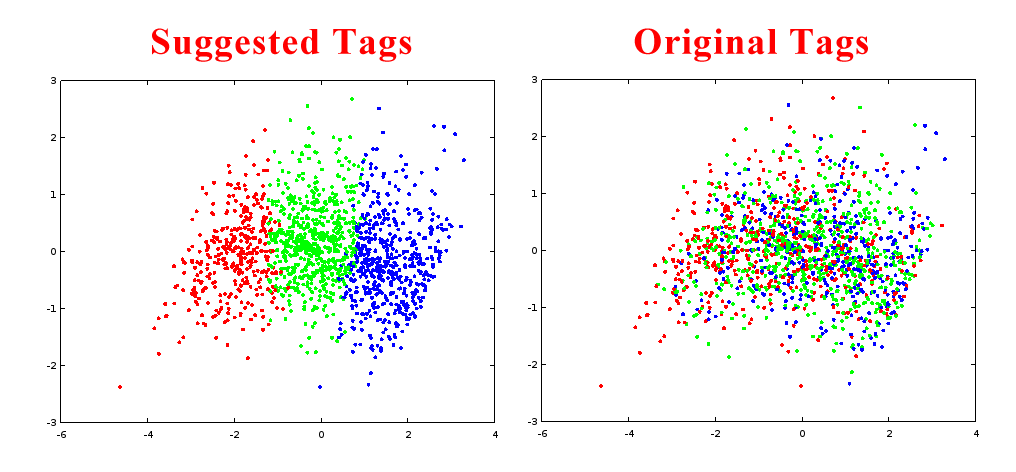
\includegraphics[width=\textwidth]{ClusteringOutput}
	\end{figure}
	
	\begin{center}
	\begin{table}[h]
		\begin{tabular}{ | m{2cm} | m{1.7cm} | m{1.3cm} | m{1.3cm} | m{1.5cm} | m{1.3cm} | m{1.3cm} | m{1.3cm} | }
		\hline
		\textbf{Feature} & \textbf{Level} & \textbf{Min} & \textbf{Q1} & \textbf{Median} & \textbf{Q3} & \textbf{Max} & \textbf{Mean}\\ 
		\hline
		\textbf{Feature 1} & \textbf{Easy Medium Hard} & -0.515 \hspace{5mm}-1.359 \hspace{5mm}-1.686 & 0.842 \hspace{5mm}-0.470 \hspace{5mm}-1.213 & 1.370  \hspace{5mm}-0.106 \hspace{5mm}-0.946 & 1.818 \hspace{5mm}0.373 \hspace{5mm}-0.605 & 2.934 \hspace{5mm}1.813 \hspace{5mm}1.106 & 1.318 \hspace{5mm}-0.031 \hspace{5mm}-0.860\\
		\hline
		\textbf{Feature 2} & \textbf{Easy Medium Hard} & -0.342 \hspace{5mm}-0.842 \hspace{5mm}-1.843 & 0.962 \hspace{5mm}-0.018 \hspace{5mm}-1.843 & 1.159  \hspace{5mm}0.409 \hspace{5mm}-1.092 & 1.159 \hspace{5mm}0.730 \hspace{5mm}-0.642 & 1.159 \hspace{5mm}1.159 \hspace{5mm}0.159 & 1.018 \hspace{5mm}0.377 \hspace{5mm}-1.139\\
		\hline
		\textbf{Feature 3} & \textbf{Easy Medium Hard} & -4.498 \hspace{5mm}-1.667 \hspace{5mm}-2.050 & -1.631 \hspace{5mm}-0.339 \hspace{5mm}0.159 & -1.091  \hspace{5mm}0.028 \hspace{5mm}0.589 & -0.623 \hspace{5mm}0.479 \hspace{5mm}1.132 & 1.104 \hspace{5mm}2.620 \hspace{5mm}3.380 & -1.134 \hspace{5mm}0.093 \hspace{5mm}0.662\\
		\hline
		\end{tabular}
		\caption{Statistics for k-Means Output}
	\end{table}
	\end{center}
	
	\paragraph{Estimated Manual Tagging Accuracy: 43.73\%}
	
	
	% Describe Competitive Learning
	\newpage
	\subsubsection{Competitive Learning}
	Competitive Learning is another unsupervised learning algorithm which can
	be used for	clustering of data. This algorithm can be implemented as
	a neural network. Autoencoder was used to encode features to feed input
	to the algorithm. Following two features were fed to autoencoder:
	\begin{enumerate}
	\item Fraction of people who solved a question correctly.
	\item Fraction of people in top five percentile who solved the question
	correctly.
	\end{enumerate}
	
	Best results were obtained when only these two features were used, 
	although other feature combinations were also tried. This algorithm
	is also faster than k-Means	clustering. Output has been shown below:
	\begin{figure}[h]
	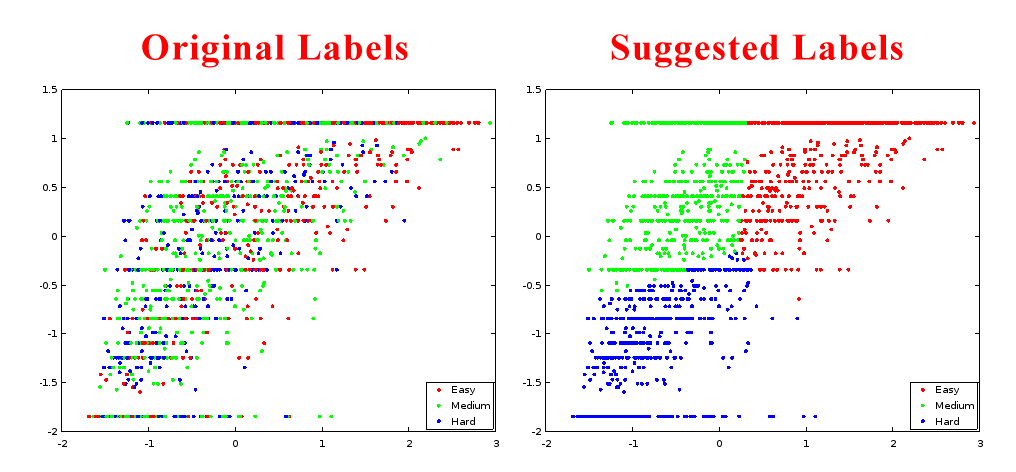
\includegraphics[width=\textwidth]{CompetitiveOutput}
	\end{figure}
	
	\begin{center}
	\begin{table}[h]
		\begin{tabular}{ | m{2cm} | m{1.7cm} | m{1.3cm} | m{1.3cm} | m{1.5cm} | m{1.3cm} | m{1.3cm} | m{1.3cm} | }
		\hline
		\textbf{Feature} & \textbf{Level} & \textbf{Min} & \textbf{Q1} & \textbf{Median} & \textbf{Q3} & \textbf{Max} & \textbf{Mean}\\ 
		\hline
		\textbf{Feature 1} & \textbf{Easy Medium Hard} & 0.234 \hspace{5mm}-1.503 \hspace{5mm}-1.686 & 0.652 \hspace{5mm}-0.695 \hspace{5mm}-1.211 & 1.051  \hspace{5mm}-0.419 \hspace{5mm}-0.886 & 1.580 \hspace{5mm}-0.096 \hspace{5mm}-0.414 & 2.934 \hspace{5mm}0.324 \hspace{5mm}1.106 & 1.169 \hspace{5mm}-0.412 \hspace{5mm}-0.781\\
		\hline
		\textbf{Feature 2} & \textbf{Easy Medium Hard} & -0.642 \hspace{5mm}-0.556 \hspace{5mm}-1.843 & 0.492 \hspace{5mm}-0.042 \hspace{5mm}-1.843 & 1.159  \hspace{5mm}0.409 \hspace{5mm}-1.092 & 1.159 \hspace{5mm}0.859 \hspace{5mm}-0.717 & 1.159 \hspace{5mm}1.159 \hspace{5mm}-0.175 & 0.804 \hspace{5mm}0.392 \hspace{5mm}-1.185\\
		\hline
		\end{tabular}
		\caption{Statistics for Competitive Learning Output}
	\end{table}
	\end{center}
	
	\paragraph{Estimated Manual Tagging Accuracy: 43.05\%}
	
	
	% Describe EM
	\newpage
	\subsubsection{Expectation Maximization Algorithm}
	Expectation Maximization algorithm can be used for \textit{soft clustering}.
	of the data. For this algorithm, a mixture of gaussians model was assumed.
	From the obtained soft clustering output, question labels were predicted
	by taking most likely tag for each question. The following features were used:
	\begin{enumerate}
	\item Fraction of people who solved a question correctly.
	\item Fraction of people in top five percentile who solved the question
	correctly.
	\end{enumerate}
	
	Best results were obtained when only these two features were used, 
	although other feature combinations were also tried. This algorithm provides
	a skewed output forcing many questions to fall in the medium difficulty
	level category. Output has been shown below:
	\begin{figure}[h]
	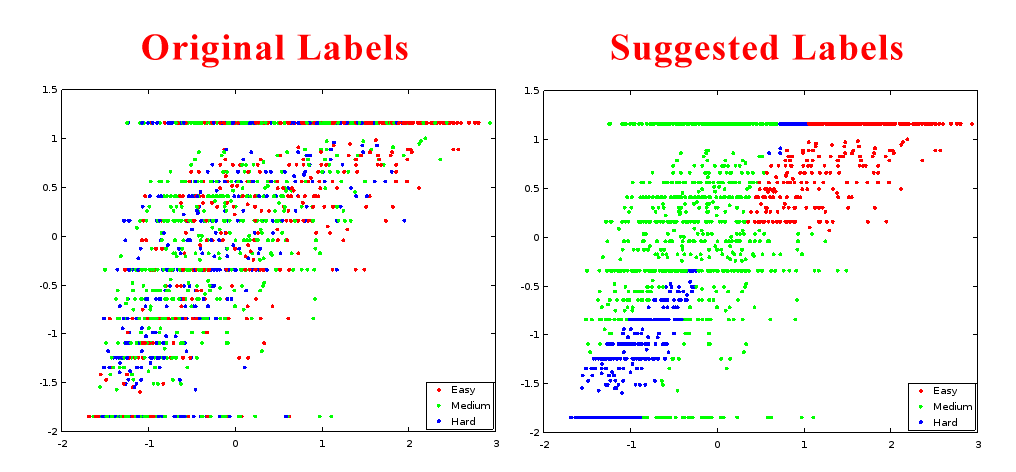
\includegraphics[width=\textwidth]{EMOutput}
	\end{figure}
	
	\begin{center}
	\begin{table}[h]
		\begin{tabular}{ | m{2cm} | m{1.7cm} | m{1.3cm} | m{1.3cm} | m{1.5cm} | m{1.3cm} | m{1.3cm} | m{1.3cm} | }
		\hline
		\textbf{Feature} & \textbf{Level} & \textbf{Min} & \textbf{Q1} & \textbf{Median} & \textbf{Q3} & \textbf{Max} & \textbf{Mean}\\ 
		\hline
		\textbf{Feature 1} & \textbf{Easy Medium Hard} & 0.355 \hspace{5mm}-1.519 \hspace{5mm}-1.686 & 0.986 \hspace{5mm}-0.671 \hspace{5mm}-1.250 & 1.412  \hspace{5mm}-0.265 \hspace{5mm}-0.979 & 1.824 \hspace{5mm}0.137 \hspace{5mm}-0.576 & 2.934 \hspace{5mm}1.485 \hspace{5mm}1.031 & 1.415 \hspace{5mm}-0.271 \hspace{5mm}-0.762\\
		\hline
		\textbf{Feature 2} & \textbf{Easy Medium Hard} & 0.068 \hspace{5mm}-1.843 \hspace{5mm}-1.843 & 0.559 \hspace{5mm}-0.342 \hspace{5mm}-1.843 & 0.971  \hspace{5mm}0.159 \hspace{5mm}-1.242 & 1.159 \hspace{5mm}0.659 \hspace{5mm}-0.717 & 1.159 \hspace{5mm}1.159 \hspace{5mm}1.159 & 0.846 \hspace{5mm}0.081 \hspace{5mm}-0.983\\
		\hline
		\end{tabular}
		\caption{Statistics for EM Output}
	\end{table}
	\end{center}
	
	\paragraph{Estimated Manual Tagging Accuracy: 45.40\%}
	
	
	% Describe Weighted Clustering
	\newpage
	\subsubsection{Weighted Clustering}
	The core idea behind using weighted clustering is to allow students
	who have got higher scores to contribute more towards clustering as
	compared to those students who have got lower scores. The rationale
	behind using such a strategy is that students with higher scores give
	more authentic data containing fewer random guesses. The following
	weighted features were used with k-Means Clustering to achieve weighted
	clustering:
	\begin{enumerate}
	\item Fraction of people who solved a question correctly adjusted by weight.
	\item Average weight adjusted marks of students who did not attempt a given 
	question or solved it incorrectly.
	\end{enumerate}
	
	Weighing of features is used by assigning higher weights to students who
	have got higher scores and vice versa. This in effect gives rise to a 
	weighted clustering algorithm without changing the core algorithm. One
	difficulty is estimating the accuracy of suggested tags since now we
	are no longer dealing with original features, hence result analysis has been
	done using original features from k-Means Clustering.
	\begin{figure}[h]
	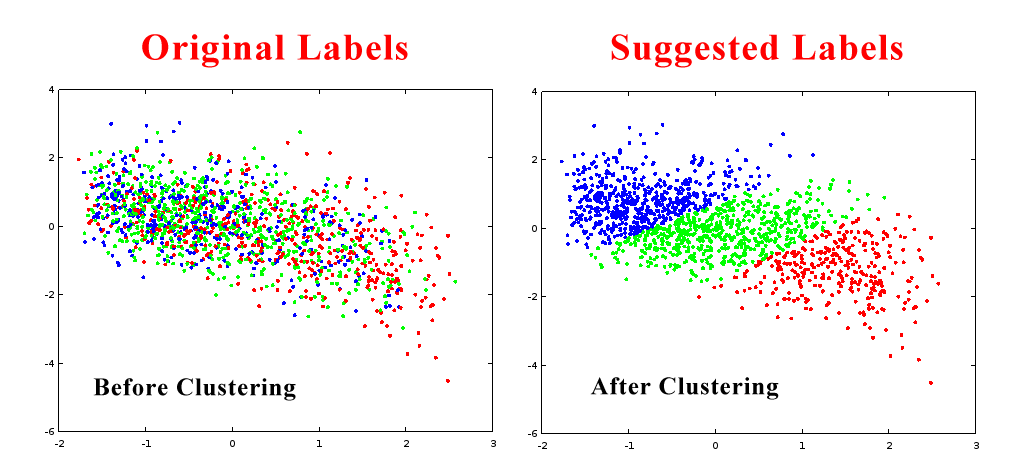
\includegraphics[width=\textwidth]{WeightedClusteringOutput}
	\end{figure}
	
	\begin{center}
	\begin{table}[h]
		\begin{tabular}{ | m{2cm} | m{1.7cm} | m{1.3cm} | m{1.3cm} | m{1.5cm} | m{1.3cm} | m{1.3cm} | m{1.3cm} | }
		\hline
		\textbf{Feature} & \textbf{Level} & \textbf{Min} & \textbf{Q1} & \textbf{Median} & \textbf{Q3} & \textbf{Max} & \textbf{Mean}\\ 
		\hline
		\textbf{Feature 1} & \textbf{Easy Medium Hard} & -0.515 \hspace{5mm}-1.504 \hspace{5mm}-1.686 & 0.907 \hspace{5mm}-0.447 \hspace{5mm}-1.188 & 1.424  \hspace{5mm}-0.013 \hspace{5mm}-0.883 & 1.851 \hspace{5mm}0.483 \hspace{5mm}-0.506 & 2.934 \hspace{5mm}2.165 \hspace{5mm}1.485 & 1.380 \hspace{5mm}0.040 \hspace{5mm}-0.802\\
		\hline
		\textbf{Feature 2} & \textbf{Easy Medium Hard} & -1.843 \hspace{5mm}-1.843 \hspace{5mm}-1.843 & 1.159 \hspace{5mm}-0.183 \hspace{5mm}-1.468 & 1.159  \hspace{5mm}0.409 \hspace{5mm}-0.842 & 1.159 \hspace{5mm}0.826 \hspace{5mm}-0.342 & 1.159 \hspace{5mm}1.159 \hspace{5mm}1.159 & 1.020 \hspace{5mm}0.238 \hspace{5mm}-0.818\\
		\hline
		\textbf{Feature 3} & \textbf{Easy Medium Hard} & -4.498 \hspace{5mm}-1.850 \hspace{5mm}-1.121 & -1.733 \hspace{5mm}-0.494 \hspace{5mm}0.379 & -1.127  \hspace{5mm}0.136 \hspace{5mm}0.741 & -0.731 \hspace{5mm}0.198 \hspace{5mm}1.238 & 0.481 \hspace{5mm}1.979 \hspace{5mm}3.380 & -1.227 \hspace{5mm}-0.137 \hspace{5mm}0.822\\
		\hline
		\end{tabular}
		\caption{Statistics for EM Output (Using Features from k-Means Clustering)}
	\end{table}
	\end{center}
	
	\paragraph{Estimated Manual Tagging Accuracy: 43.18\%}
	
	% Discuss the results obtained for part 2
	\subsection{Performance Prediction Problem}
	Different algorithms were implemented for solving the
	\textit{Performance Prediction Problem}. Four of these were classification
	algorithms and one was a regression algorithm. The results obtained have
	been described below, beginning with a description of features that have
	been used:
	
	% Discuss Features
	\subsubsection{Features}
	\label{features}
	Following features were used for training various algorithms:
	
	\begin{enumerate}
		\item Year in college. For example, $3^{rd}$ year student
		\item Branch. For example, Computer Science and Engineering
		\item Gender
		\item State to which student belongs
		\item Region to which student belongs
		\item College to which student belongs
		\item Role of Student. Team Leader or Team Member
	\end{enumerate}
	
	It is to be noted that all these are categorical features Further
	there are different number of categories possible for each of these
	features. In order to deal with categorical features we have adopted
	the widely popular technique of \textbf{feature binarization}.\newline
	
	In feature binarization each categorical feature is turned into a vector
	of binary features. One binary feature is present per category and this
	binary feature tests whether the given example belongs to that category or
	not.\newline
	
	In order to deal with missing category information and unseen category
	values in the test set, a separate category called \textit{other} is
	included with each feature.

	
	% Discuss Linear Regression 
	\subsubsection{Linear Regression}
	Linear Regression is often viewed as the simplest machine learning algorithm.
	Despite being very simple, this is one of the most powerful learning
	algorithm. If we want to predict the exact marks that a student might
	get instead of assigning a class to each student, linear regression is
	the perfect candidate.\newline
	
	All the features described in [Features section \ref{features}] were used. The
	mean square error per test example was found to be 68.53 when 5\% of
	the data was used as test data. This translates to an error of 8.28
	marks per test example. It was also found that the average standard deviation
	from mean is 8.405 even when all the features except gender and role
	are same. Hence the results of linear regression are satisfactory given
	the data that we had.
	
	\newpage
	
	% Discuss SVM
	\subsubsection{Support Vector Machine}
	Support Vector Machines or SVMs are considered to be the most effective
	off-the-shelf classifiers. To use a classification algorithm like SVM, 
	we divided the marks obtained by various students into various class
	intervals and assigned the corresponding class to each student. Thus
	the goal was to predict the class to which a student belongs.\newline
	
	A highly optimized software library for training and using SVMs called
	\textbf{libsvm}\cite{libsvm} was used. The training time of this 
	algorithm was greater than that of any other algorithm that has been
	implemented for \textit{Performance Prediction Problem}.\newline
	
	On the test set, an accuracy in the range of 10\% to 13\% was obtained
	when 5\% of the data was used as the test set. The output was strange
	in the sense that SVM predicted that all the students in the test set
	belong to class 9, which is the mean class. Even with such an extreme
	output, we obtained better accuracy than what we will get if we randomly assign
	classes. \newline
	
	This output serves as a control. By using a widely used off-the-shelf
	library we ensured that there is no bug in the implementation of SVM.
	Thus the strange output signifies that classification is very difficult
	given the current data. The correlation between the profile of student 
	and his/her performance is very low, not enough to predict anything else
	except the mean class.
	
	
	% Discuss the Naive Bayes Algorithm
	\subsubsection{Naive Bayes}
	Naive Bayes algorithm is an effective algorithm that is used for probabilistic
	classification. It is based on Bayes' rule. This algorithm makes an 
	underlying assumption of conditional independence which is known as the
	Naive Bayes assumption.\newline
	
	\begin{figure}[h]
	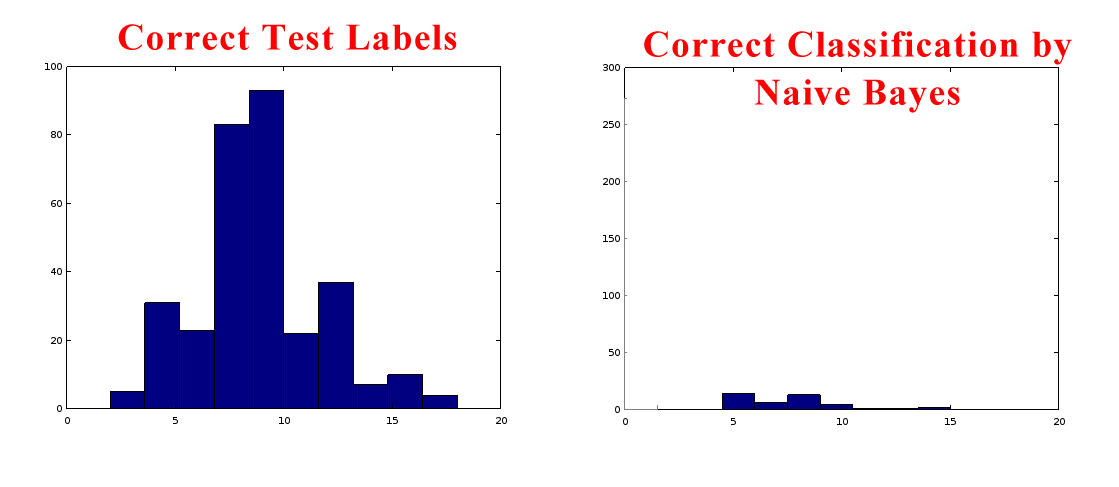
\includegraphics[width=\textwidth]{CorrectVsNaiveBayes}
	\end{figure}
	
	The problem was turned into a classification problem by dividing marks
	obtained into class intervals as it was done for Support Vector Machine.
	One important detail that separates this algorithm from other classification
	algorithms that have been implemented for \textit{Performance Prediction}
	problem is that we have not used feature binarization. Since feature binarization
	was the bottleneck of performance for other algorithms, this algorithm
	runs much faster.
	
	\paragraph{Accuracy on Test Set: 13\% - 18\%\newline}
	
	It was also observed that while other classification algorithms tend
	to predict only those class labels which are closer to mean, this
	algorithm gave a more distributed and realistic class label output.
	It was not selected as the final algorithm because Neural Networks
	were providing a higher accuracy in general.	
	
	
	% Discuss the Neural Network with One Hidden Layer
	\subsubsection{Neural Network with Single Hidden Layer}
	Neural Networks can be used as very powerful non-linear classifiers.
	Two different neural networks were implemented with different number
	of hidden layers. This section describes the neural network with a
	single hidden layer.\newline
	
	\begin{figure}[h]
	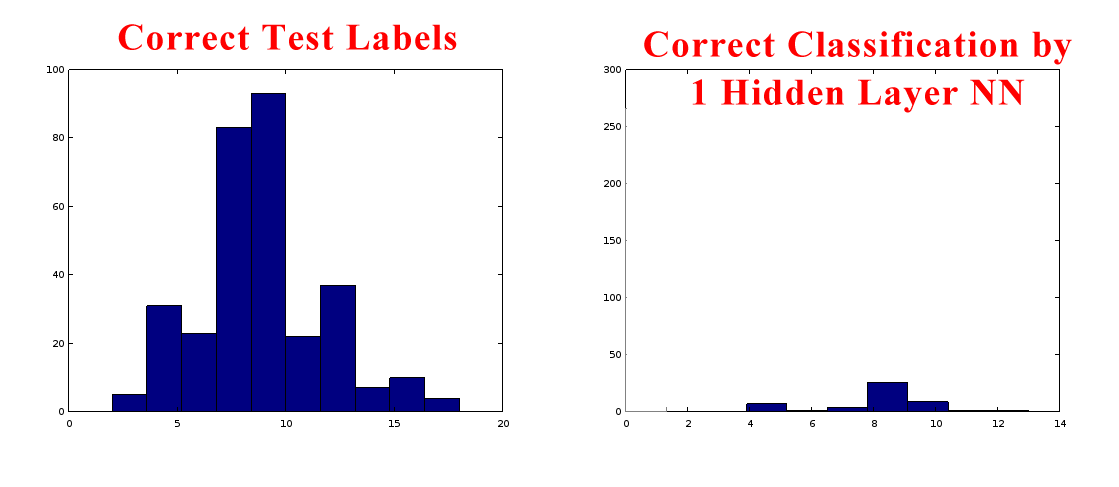
\includegraphics[width=\textwidth]{CorrectVsNN1}
	\end{figure}
	
	After formulating the problem as a classification problem as it was
	done in case of SVMs, the single layer neural network was made. It
	had 148-151 input units depending on the output of PCA, 35 hidden
	units and 20 output units, one for each class.
	
	\paragraph{Accuracy on Test Set: 15\% - 20\%\newline}
	
	This output was obtained when 5\% of the data was used as test set and
	99\% of variance was retained by PCA.
	Accuracy increases up to 48\% if we allow an error of one neighboring
	class during classification. This implementation gives a balance between
	accuracy and complexity, hence this was chosen as the final algorithm.	
	
	
	% Discuss the Neural Network with Two Hidden Layers
	\subsubsection{Neural Network with Two Hidden Layers}
	Another neural network with two hidden layers was implemented to as
	an attempt to increase the accuracy by making the model more complex.
	This two hidden layer neural network has been described in this section.
	\newline
	
	\begin{figure}[h]
	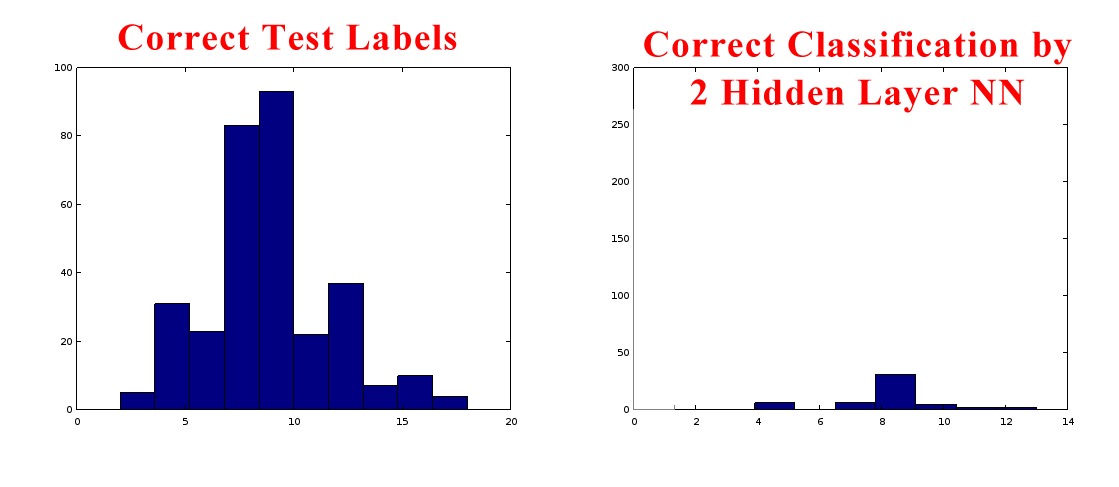
\includegraphics[width=\textwidth]{CorrectVsNN2}
	\end{figure}
	
	After formulating the problem as a classification problem as it was
	done in case of SVMs, the two layer neural network was made. It
	had 148-151 input units depending on the output of PCA, and two 
	hidden layers containing 25 hidden units each. The output layer
	consisted of 20 units, one for each class. The total number of free
	parameters in this model, i.e. the total number of weights that can
	be changed is about 4900, hence this network is more prone to 
	overfitting.
	
	\paragraph{Accuracy on Test Set: 15\% - 20\%\newline}
	
	This output was obtained when 5\% of the data was used as test set and
	99\% of variance was retained by PCA.
	In general, the accuracy of this network is more than the accuracy of 
	the neural network with a single hidden layer but the difference is not
	much (approx. 1\%). Since this model increases the complexity of the
	model but not lead to any significant increase in accuracy, it is advisable
	to use the single hidden layer neural network.
	
	
	% Discuss the Bugs
	\section{Known Bugs}
	\begin{enumerate}
		\item plotData function in all algorithms crashes if only 1 feature is chosen.
		\item Only 1489 questions out of 1500 have been classified. For the remaining questions:
		\begin{enumerate}
			\item Two questions were solved by all people and hence are definitely easy.
			These 2 questions are:
			\begin{enumerate}
				\item 199
				\item 1350
			\end{enumerate}
			\item Eight questions were solved by none and hence are definitely hard.
			These 8 questions are:
			\begin{enumerate}
				\item 206
				\item 377
				\item 378
				\item 1029
				\item 1038
				\item 1143
				\item 1257
				\item 1386
			\end{enumerate}
			\item One question was never presented to any person in top 5 percentile.
			(This question has been classified by weighted clustering) 
		\end{enumerate}
		\item The regression algorithm using Neural Network has a very poor
		convergence rate. The gradients generated are very small which cause
		the algorithm to stop before convergence.
	\end{enumerate}
	
	
	% Discuss Future Work
	\section{Future Work}
	Some of the proposed projects that can be built using the results of
	this projects are as follows:
	
	\subsection{Suggesting Study Material}
	If every question is assigned to one of the categories, then
	we can reverse the process to classify students based on the type
	of questions that they have solved. This will help in suggesting 
	appropriate study material to students. For example some students
	did very well in calculus and performed poorly in complex numbers,
	then they should be suggested the study material focused on complex
	numbers.
	
	\subsection{Noise Removal}
	Once correct difficulty tags are known, this information can be used
	to detect random guesses made by the students which will reduce noise
	in data obtained from subsequent iterations of the test. Now this filtered
	data can be used to further improve the accuracy of assigned difficulty
	levels. This is just like Expectation Maximization algorithm spread
	in time. By detecting random guesses an improved performance estimate
	can be made for each student which can be used for selecting students
	instead of using the raw score.
	
	\subsection{More Intelligent Performance Prediction}
	One major problem with performance prediction was non-availability
	of relevant data. The correlation between available data and performance
	of students was very poor. By gathering data pertaining to the academic
	performance of students in the past, a more intelligent Performance 
	Prediction system can be designed.
	
	\nocite{*}	
	
	\newpage
	\printbibliography[heading=bibintoc]

\end{document}
